\todoNow{Write this:} the data analysis of this project is to calibrate and to extract rv.

\subsection{Calibration} 

    The calibration is needed to map each pixel on the CCD to a specific wavelength. Such a map is referred to as a wavelength solution. To do this, we need a light source with known frequencies, preferably many discrete peaks. EXPRES uses a Thorium Argon lamp for an initial trial wavelength solution and then a laser frequency comb (LFC) for an more precise solution.
    
    The Thorium Argon lamp produces 4,000 lines across 82 orders, which can be identified and mapped to a wavelength through a \emph{line atlas}. An intial wavelength solution for all pixels is then produced by linear interpolation. (In this project I have not done this calibration).

    The LFC generates a series of evenly spaced spectral lines, typically 20,000 lines across 50 orders. The range of the LFC is thus shorter, and for this reason the ThAr exposures can also be used for a rough calibration outside the LFC range. The frequencies of the LFC lines are given by the relation
    
    \begin{equation}
        \label{eq:LFC_freq_eq}
        v_{n}=v_{\text{rep}} \times n+v_{\text{offset}}
    \end{equation}

    for integers $n$. The repetition rate $v_{\text {rep }}$ and offset frequency $v_{\text {offset }}$ are referenced against a GPS-disciplined quartz oscillator, providing calibration stability corresponding to a fractional uncertainty of less than $8 \times 10^{-12}$ for integration times greater than 1s. (p. 8, \cite{first_RV_from_EXPRES}). The values I have used in the calibration, $v_{\text{rep}} = 14e9$ and $v_{\text{offset}} = 6.19e9$, were provided by Lars Buchhave. See figure \ref{fig:LFC_CCD} right side for a plot of the intensities measured across the CCD.

    \begin{SCfigure}[1][!ht]%
        \begin{wide}  
            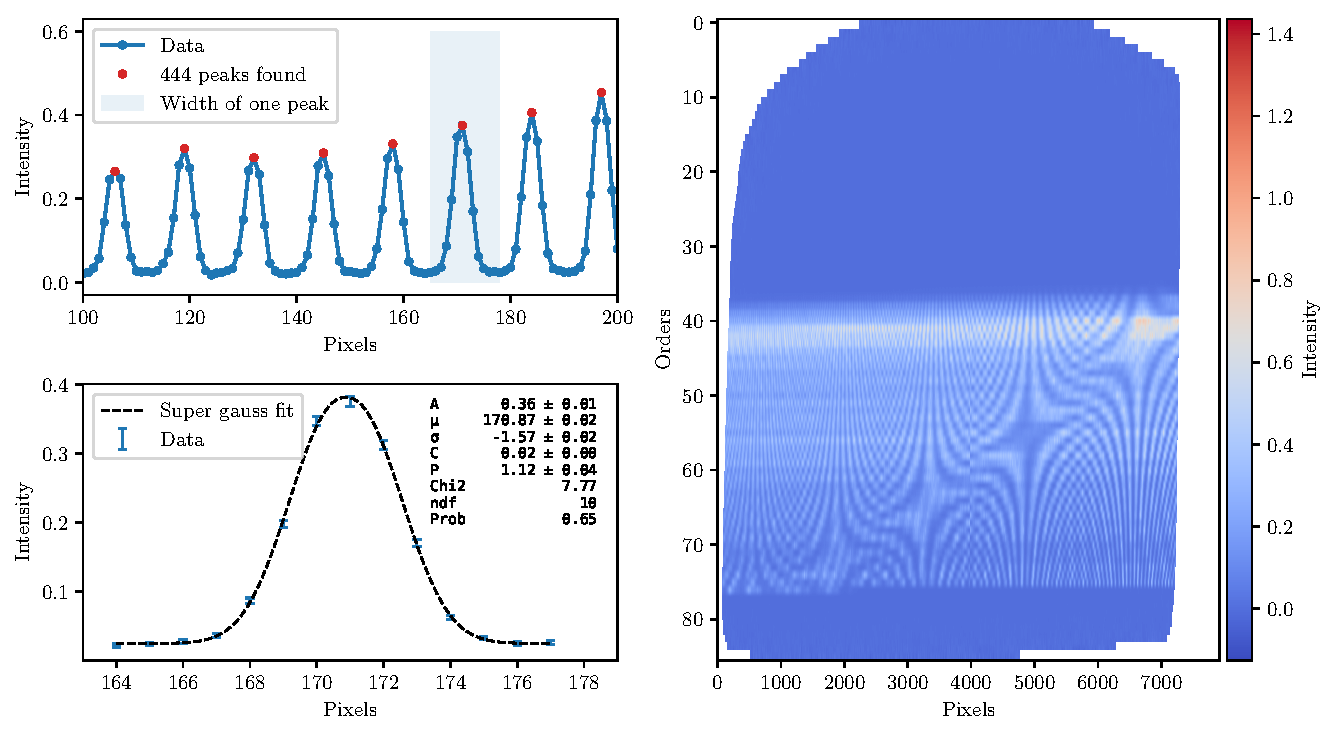
\includegraphics[width=\textwidth]{figures/LFC_peak_fitting_overview.pdf}
            \caption{Right: Measured intensities for the LFC across the CCD (unitless). Upper left: illustration of a few LFC lines in order 65. Peaks are identified with scipy peak finder. Lower left: each peak is fitted with a super gauss to find the exact top of the peak with uncertainties.}
            \label{fig:LFC_CCD}
        \end{wide}
    \end{SCfigure}

    The following procedure is followed to determine the location of the LFC lines on the CCD: 1) Find peaks using scipy peak finder, 2) make data slices around each peak with the size of the average distance between peaks, 3) using iminuit do a chi2 minimisation fit to each peak with a super-gauss plus a linear background. See figure \ref{fig:LFC_CCD} left side.

    A super-gauss, defined in equation \ref{eq:LFC_super_gauss}, is a regular gaussian but with an extra parameter, here denoted $P$, that allows the top of the gaussian to be flattened. The last two terms here add a linear background and an offset. 
    
    \begin{equation}
        \label{eq:LFC_super_gauss}
        f(x ; A, B, C, P, \mu, \sigma) = A \exp \left(-\left(\frac{\left(x-\mu\right)^{2}}{2 \sigma^{2}}\right)^{P}\right) + B(x-\mu) + C
    \end{equation}

    The fit is then a standard chi2 minimization:

    \begin{equation}
        \label{eq:chi2_super_gauss}
        \chi^{2}=\sum_{i=1}^{N}\left[\frac{y_{i}-f(x ; A, B, C, P, \mu, \sigma)}{\sigma_{i}}\right]^{2}
    \end{equation}

    Where $N$ is the number of data points, $x$ is pixel-space, $y_i$ and $\sigma_i$ is the measured intensity and uncertainty respectively. The fit returns the values and uncertainties for the parameters $A, B, C, P, \mu, \sigma$ when the chi2 is minimized.
    
    We are most interested in $\mu$, which gives the position of the LFC peak on the CCD (in pixel-space). With the intial rough wavelength solution derived from the ThAr lamp (precalculated in the data set that I've used) I can determine what the approximate wavelength of the LFC peak should be. To find the better wavelength solution I then go look up the closest frequency given by eq. \ref{eq:LFC_freq_eq}. And we now have a map of ~20,000 points on the CCD with a good wavelength solution. We would however like to have a wavelength solution for all pixels on the CCD, so we need to find a way to estimate the wavelength solution in between LFC lines. To do that I have explored two approaches: polynomial fitting and cubic-spline interpolation. Before moving on though, it is worthwhile to study the chi2 values from the many fits we just performed, as they can help up evaluate whether the errors of the original data are correct.
    
    \subsubsection{Errors in the calibration data}

    According to Lily Zhao et al, the line spread function of EXPRES can best be represented by a super-gaussian \cite{yale_data}, and so as we fit a super-gaussian to the peaks, the chi2 will grow if the measured values do not agree with the predicted values within the uncertainties. For a given data point, if the measured value differs by exactly the uncertainty, that data point would contribute 1 to the sum. However, fitting with the super-gaussian (including a linear background) we also have 6 fitting parameters that allow some wiggle room for the model to fit the data, which we must compensate for. For a given data series, such as an LFC peak, we can expect the chi2 roughly equal the number of data points in the sum \emph{minus} the number of parameters in the fit, i.e. the number of the degrees of freedom:
    
    % The LFC fits files come with an uncertainty on the intensity. It appears however that this uncertainty might be a bit underestimated. We can see this by plotting the $\chi^2$- and P-values for the LFC peak super-gauss fits, as done in figure \ref{fig:calib_errors}. The $\chi^2$ value should be roughly equal to the number of degrees of freedom in the fit (eq. \ref{eq:LFC_super_gauss}), which is: 

    \begin{equation}
        \label{eq:ndof}
        N_\text{dof} = N_\text{data-points} - N_\text{fit-parameters} =  13 - 6 = 7,
    \end{equation}

    as I use roughly 13 data points in each fit (the LFC line spacing does vary a bit across the CCD). 

    So if we plot all chi2 values we get from fitting the LFC lines, as I've done in figure \ref{fig:calib_errors}, we should see a typical chi2 distribution with a peak around 7. Using the uncertainties as provided in the data file, the chi2 distribution is however very flat (red curve). It peaks somewhere around 25, which suggests that the uncertainties are about a factor $\sqrt{3}$ too small (square-root because the chi2 of course is squared and $25/3 \sim 8$), and scalling up the uncertainties by $\sqrt{3}$ and fitting the peaks again does in fact give a chi2-distribution with a peak roughly around 8.
    additionally we can also look at the p-value distribution. With proper uncertainties, we should expect neither too many awful fits (p=0) nor too many perfect fits (p=1), but rather a roughly flat distribution. Although the chi2-distribution check is more clear-cut, the p-value distribution for uncertainties scaled by $\sqrt{3}$ (green) is better. Scaling by $\sqrt{6}$ is too much: the chi2 peaks around 4 and the p-dstribution shows many more perfect fits.
                
    \begin{SCfigure}[1][!ht]%
        \begin{wide}  
            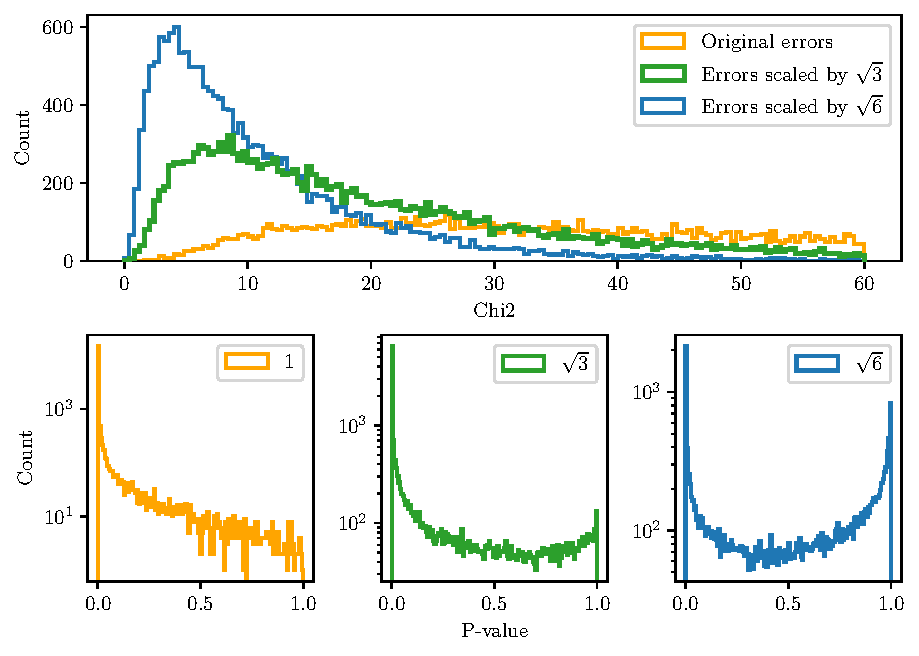
\includegraphics[width=\textwidth]{figures/calib/calib_errors2.pdf}
            \caption{Chi2-values and p-values from individual LFC peak super-gauss fits with photon count (spectrum) errors multiplied by different scale-factors (1, $\sqrt{3}$ and $\sqrt{10}$). See text for more details.}
        \label{fig:calib_errors}
        \end{wide}
    \end{SCfigure}

    \subsubsection{Poly-fit calibration}
    Since the LFC peak positions, as seen in the right plot in figure \ref{fig:LFC_CCD}, appear to exhibit a certain periodic behavour, my initial approach to compute a wavelength solution across the whole CCD was to fit the LFC peak positions with a polynomial. Looking at the residuals of fitting the LFC line positions with polynomials of increasing degree revealed smaller and smaller periodic variations, until reaching 5th degree, see figure \ref{fig:LFC_calib_poly_degrees}. The p-value drops to 0 for 6th degree, and the per line rms (\todoNow{1}) explodes. Only LFC lines with a chi2 smaller than 100 was used for the analysis and errors were scaled by $\sqrt{3}$ locating LFC lines.

    \begin{SCfigure}[1][!ht]%
        \begin{wide}  
            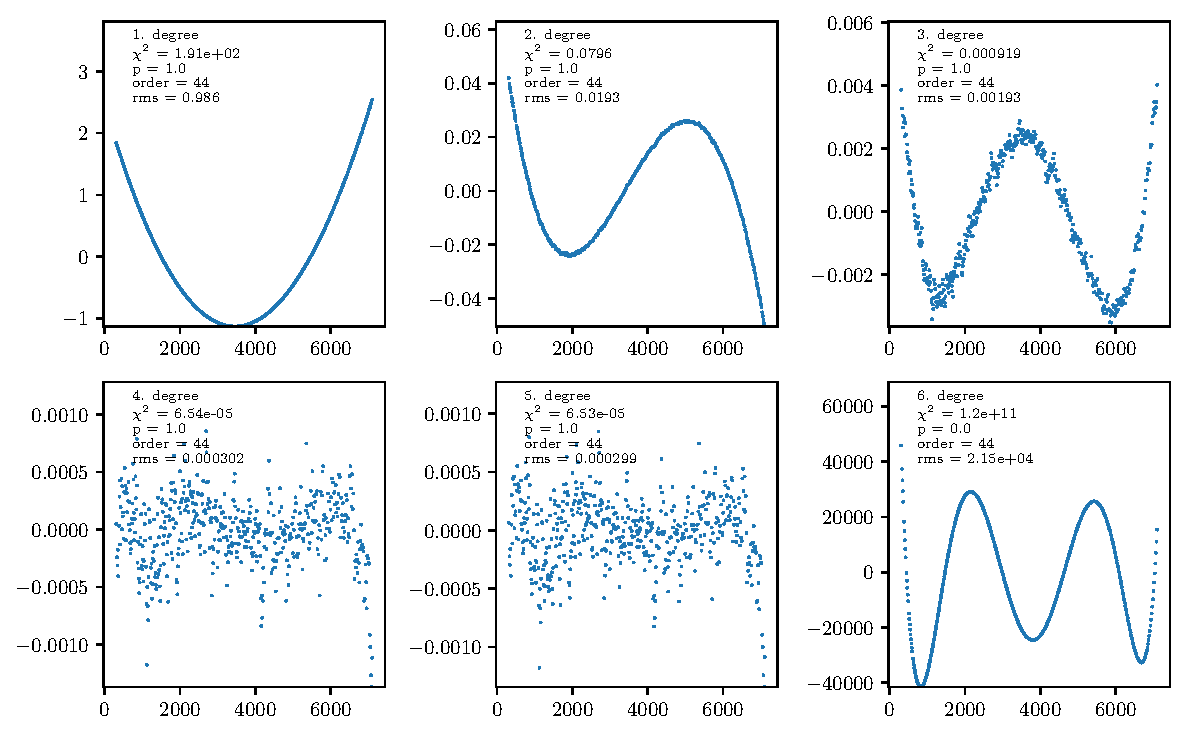
\includegraphics[width=\textwidth]{figures/calib/calib_poly_fit_degrees_order44_residuals_ang.pdf}
            \caption{Residuals from fitting LFC peak positions with polynomials of increasing degree, in order 44. Pixels on the x-axis and residuals in m/s on the y-axis. Errors used for determining peak locations have been scaled by $\sqrt{3}$.}
            \label{fig:LFC_calib_poly_degrees}
        \end{wide}
    \end{SCfigure}

    The residuals plotted show the difference between the theoretical line position given by equation \ref{eq:LFC_freq_eq} and the wavelength solution evaluated at the line position of 

    TODO:
    - JAKOB JAKOB JAKOB JAKOB JAKOB JAKOB GET THIS STRAGIHT 
    - and add this: 

    $$
        \text{RMS/line} \left[\mathrm{m} \mathrm{s}^{-1}\right]=\sqrt{\sum_{n=1}^{N} \sum_{p=1}^{P} \frac{\left[\frac{\left(\lambda_{n, p, \text { pred. }}-\lambda_{p, \text { theory }}\right)}{\lambda_{p, \text { theory }}} \times c\right]^{2}}{N \times P}}
    $$

    - and refer to it from todo 1, and in the caption
    
    
    The residuals of a wavelength solution represent the difference between the wavelength solution evaluated at the line position of a calibration line and the assigned theoretical wavelength (i.e., that from Equation (4) for the LFC lines) on a line-by-line basis in every exposure. The reported rms of a wavelength solution is therefore the per-line rms, i.e.,

    % \begin{SCfigure}[1][!ht]%
    %     \begin{wide}  
    %         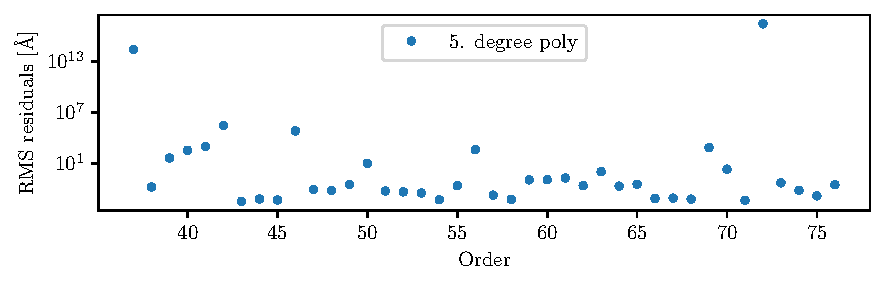
\includegraphics[width=\textwidth]{figures/calib/calib_poly_5th_res.pdf}
    %         \caption{RMS of residuals from fitting LFC peak positions with 5. degree polynomial across orders.}
    %         \label{fig:LFC_calib_5th_res}
    %     \end{wide}
    % \end{SCfigure}


    \subsubsection{Interpolation calibration}
    A cubic-spline interpolation would force all the residuals to be zero, so in order to evaluate the quality of the method, we can omit for instance every second peak from the interpolation and then compute the residual between the omitted peaks and the resulting interpolation function. Then we can flip it around and interpolate the peaks we left out before and compute the remaining residuals. 
    
    thus ending up with an array of residuals equal to the length of the results from the poly-fit method, allowing us to compare the two, as is done in figure \ref{fig:calib_poly_vs_interp}.

    The RMS of the residuals from the interpolation come out much smaller than that of the polyfit (values specified in figure \ref{fig:calib_poly_vs_interp}), in this example, suggesting that the interpolation method is superior. It is also worth noting that because the interpolation was done on only half the data points at a time, it will be even better when performed on all data points, as it would be, when used for calibrating data before an RV analysis.

    \begin{SCfigure}[1][!ht]%
        \begin{wide}  
            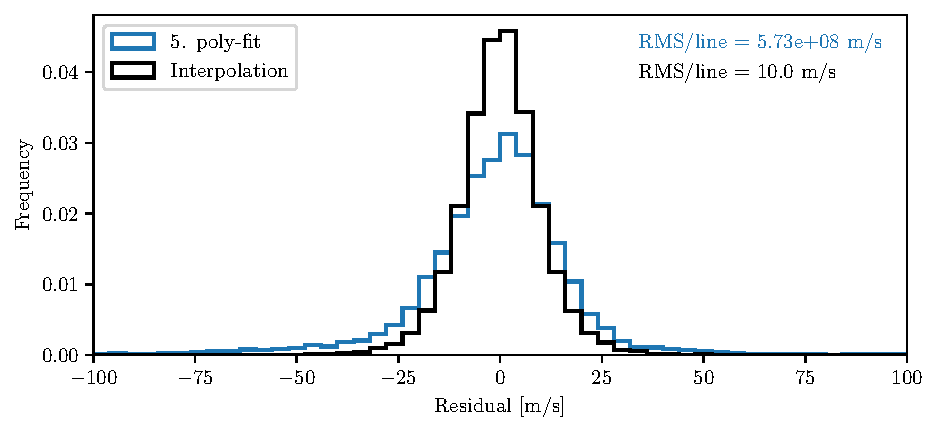
\includegraphics[width=\textwidth]{figures/calib/hist_peak_residuals_poly_and_interp.pdf}
            \caption{Residuals from calibrations performed through a 5th degree poly-fit and a cubic-spline interpolation. The per-line rms as defined in Equation (5) is given in the top-right corner in the color of the corresponding method.}
            \label{fig:calib_poly_vs_interp}
        \end{wide}
    \end{SCfigure}


\subsection{RV extraction}

    % To extract radial velocity we need to measure the doppler shift between spectra from different days of observation. The most straight-forward way to do this is to compute the cross-correlation, since, in signal processing in general, the cross-correlation is exactly a measure of the similarity of two data series as a function of the displacement of one relative to the other.

    To extract radial velocities we need to measure the doppler shift between spectra from different days of observation. One way to do that is to compute the cross-correlation, which is a measure of the similarity of two data series as a function of the displacement of one relative to the other.
    
    We can do this either for individual absorption features, chunks of the spectrum a few angstroms wide or entire orders at a time. I've chosen primarily to work with the individual features.

    Due to a lack of access to data consisting of star spectra with associated LFC captures, I've worked on RV extractions using already calibrated data provided by Lily Zhao. This data has been calibrated using a technique called excalibur \cite{zhao2021excalibur}.
    
    The data is visualized in \ref{fig:rv_data_overview}, where the top left shows an extract of wavelength vs. intensity data from an observation of HD 34411. The file also includes a model of the continuum function, with which we can normalize the spectrum through division, shown in the bottom left. On the right side is plotted all continuum normalized data within the EXCALIBUR mask, i.e. data marked as having a proper calibration.

    \begin{SCfigure}[1][!ht]%
        \begin{wide}  
            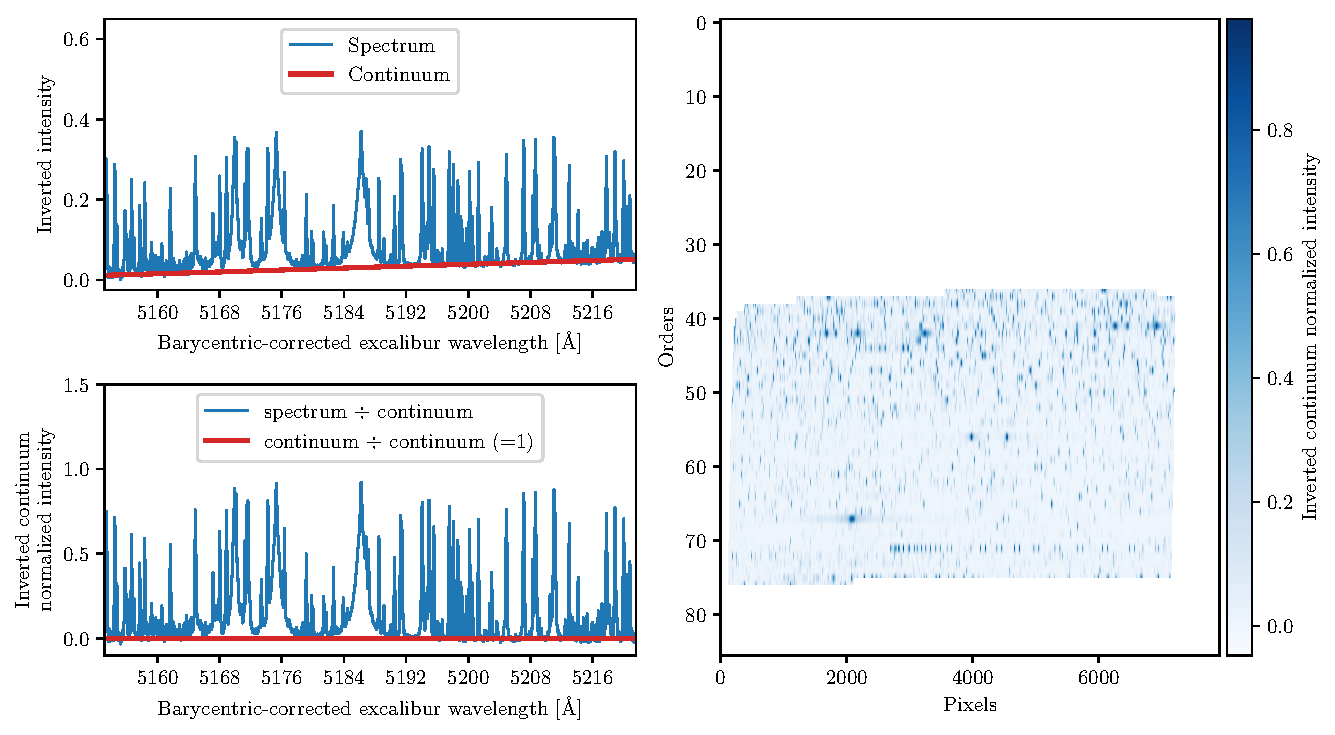
\includegraphics[width=\textwidth]{figures/rv_data_overview.pdf}
            \caption{Overview of excalibur calibrated data from an observation of HD 34411. Upper left: extract of wavelength solution vs. intensity. Lower left: continuum normalized spectrum. Right: all continuum normalized data within the excalibur mask.}
            \label{fig:rv_data_overview}
        \end{wide}
    \end{SCfigure}
            
    \subsubsection{Finding and matching features across observations}

    In order to measure how much individual absorption features move in between observations the first challenge is to find the "same" features in both observations. What follows is a quick rundown of the procedure I've devised:
    
    \begin{itemize}
        \item Load intensities from the data column \verb|"spectrum"| and errors from \verb|"uncertainty"| as well as excalibur calibrated barycentric-corrected wavelengths from \verb|"bary_excalibur"|, all masked by \verb|"excalibur_mask"|.
        \item Normalize intensities and errors with the continuum function from \verb|"continuum"|.
        \item Invert intensities to turn absorption features into positive peaks by $y = 1 - y$.
        \item Locate peaks using \verb|find_peaks| from \verb|scipy.signal| with minimum peak distance of 5 pixels and a minimum peak prominence of 0.25 (unitless).
        \item Finally slice data around each peak with a width of 30 data points. 
    \end{itemize}

    And then to match features/peaks between two observations:

    \begin{itemize}
        \item Iterate through the peaks of observations1 and find the closest peak in observation2. With excalibur calibrated data, peaks should not shift so much that they overlap. However the algorithm laid out so far does sometime match peaks that are far apart or do not resemble each other in shape at all. To bypass such matches we can add two filters:
        \begin{itemize}
            \item Maximum peak distance: We could filter out all matches where the distance between the peaks is equivalant to a radial velocity greater than 12.5 m/s (the RV Jupiter induces in the Sun). However, since we are dealing with discrete data, the difference sometimes comes out much larger than it actually is and a narrow cut of 12.5 m/s would remove many good matches. Instead setting a very generous cut of 0.5 Å, equivalant to about 20-30 km/s depending on the wavelength, filters out the few very bad matches, but leaves the rest. When analyzing non-barycentric-corrected data, I set this up to 1Å. 
            
            \item Maximum difference between the areas under the graph of two features (the sum of the intensity values in the feature): Peaks with similar shapes will give a low difference. This filter is most useful when analyzing non-barycentric-corrected, where features often move so much that they overlap. In figure \ref{fig:good_match_bad_match} is plotted an example of a bad and a good match, where the bad match can be avoided by setting the max area difference down to 0.1 (unitless). 
        \end{itemize}
        \item I've not yet devised any formal way to determine the best choice of these filters.
    \end{itemize}

    % \begin{SCfigure}[1][!ht]%
    %     \begin{wide}  
    %         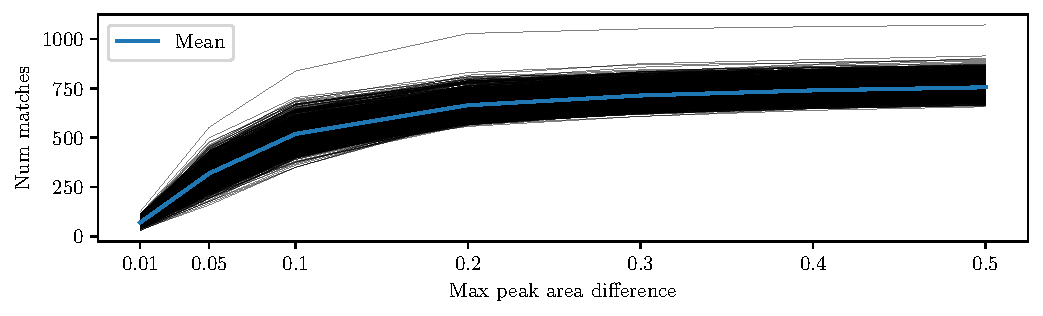
\includegraphics[width=\textwidth]{figures/max_peak_area_diff_vs_Nmatches.pdf}
    %         \caption{Average number of matches found as a function of max peak area difference for all features in observations for HD 34411.}
    %         \label{fig:max_area_diff_vs_n_matches}
    %     \end{wide}
    % \end{SCfigure}

    \begin{SCfigure}[1][!ht]%
        \begin{wide}  
            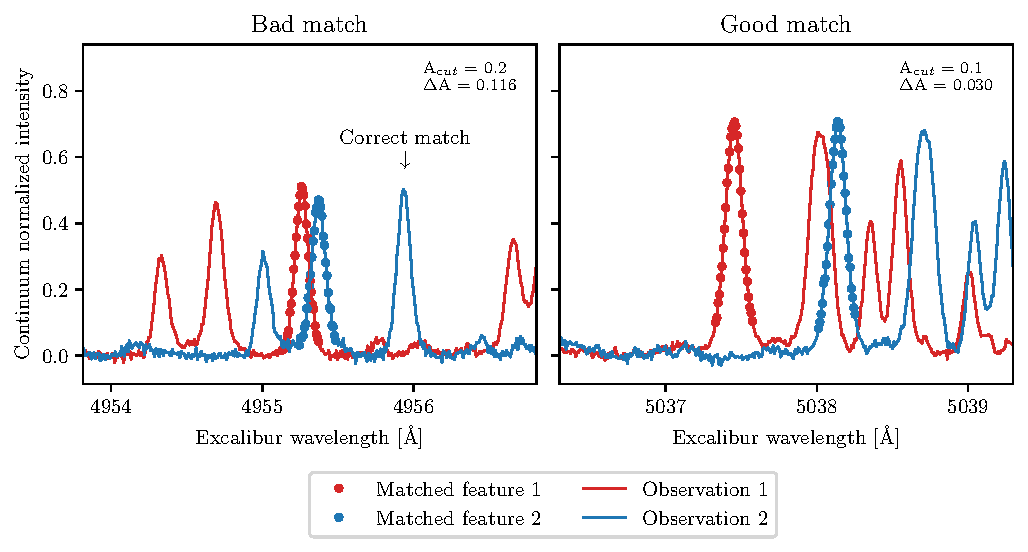
\includegraphics[width=\textwidth]{figures/good_match_bad_match.pdf}
            \caption{Example of match filtering with non-barycentric-corrected data, where features move a lot. The maximum area difference cut was set to 0.2 and 0.1 one the left and right plot repsectively. The cut on the left plot was not strict enough to avoid the bad match that was made, with a an area difference of 0.116. While on the right plot, the correct feature was selected spite another feature being closer in wavelength.}
            \label{fig:good_match_bad_match}
        \end{wide}
    \end{SCfigure}

    \subsubsection{Computing velocity shift as the cross correlation}

    At this point, I have a list of matching features in different observations. The cross-correlations will be performed as a chi2 minimization fit to find the radial velocity that for each match correctly shifts one feature onto the other one.
    
    Before moving on though, we have to cubic-spline interpolate the spectra data. I do this for two reasons: 1) the shifts we are looking for are much smaller than the individual pixels on the CCD, so we need to be able to shift by sub-pixel amounts, and 2) in order to compute the difference in intensity values between peaks, the intensity values must have the same wavelength solution, but, since EXPRES is calibrated independently for each observation, the wavelength solutions are different.
    
    So I cubic-spline interpolate the spectra data from the first observation in the match, but before interpolating the second observation, I shift the wavelength solution by multiplying the shift factor from equation \ref{eq:our_doppler}. Now I can evaluate the two interpolation functions on a common wavelength range, using $N=1000$ steps\footnote{1000 steps appeared as the best balance between run time and resulting uncertainty. See figure \ref{fig:err_vs_run_time} in appendix \ref{appendix:RV_extraction}}, and I am ready to compute the chi2:
        
    \begin{equation}
        \label{eq:shift_fit_chi2}
        \chi^{2}=\sum_{i=1}^{N}\left[\frac{y_{i}-f(x; v)}{\sigma_{i}}\right]^{2}
    \end{equation}
    
    where $y_i$ are the unshifted interpolated intensity from the first observation, $\sigma_i$ are the errors on the intensity of the first observation also sampled through a cubic-spline interpolation, and the function $f(x; v)$ is the cubic-spline interpolation function given by interpolating the intensity values of the second observation with wavelength values shifted by equation \ref{eq:our_doppler}, evaluated on the wavelength range common to both features: 
    
    \begin{equation}
        f(x; v) = \textbf{interp}[x \times ( 1 + v/c), y]\,(x_\text{common})
    \end{equation}
    
    I then compute the cross-correlation and obtain the radial velocity, $v$, as a minimization of eq (\ref{eq:shift_fit_chi2}) using iminuit for one feature. 
    
    \subsubsection{Computing velocity shifts for all features}

    We can now find and compute the cross-correlation for all feature matches between two observations. In general I find between 500-1000 matches between two observations, which results in a fair amount of statistics. The computed radial velocities do build up a normal distribution around a central value, but there are many outliers. This is due to primarily two things: 1) Bad matches making it through the selection filters, and 2) stellar activity, which are various processes on the star that cause absorption features to shift independently.
    
    This is one place where there is definite room for improvement. A better matching algorithm could supposedly be developed, but when it comes to sorting through lines affected by stellar activities, one could imagine that machine learning might be applicable. More on this in the discussion.

    For now, I've experienced with settings different cuts both in radial velocity and chi2 to weed out the bad ones, but what I've found to work the best, is simply taking the median instead of the weighted average or the mean, as the median is much less affected by outliers than both. And as there is no reason to believe that stellar activity would cause more RV outliers in one particular direction, the spread can be assumed to be symmetric and thus the median is a good approximation. In figure \ref{fig:median-mean-weighted-average} is plottet an example, which also contains at least one bad match on the far left and a constellation of features likely to be affected by stellar activity on the far right.

    \begin{SCfigure}[1][!ht]%
        \begin{wide}  
            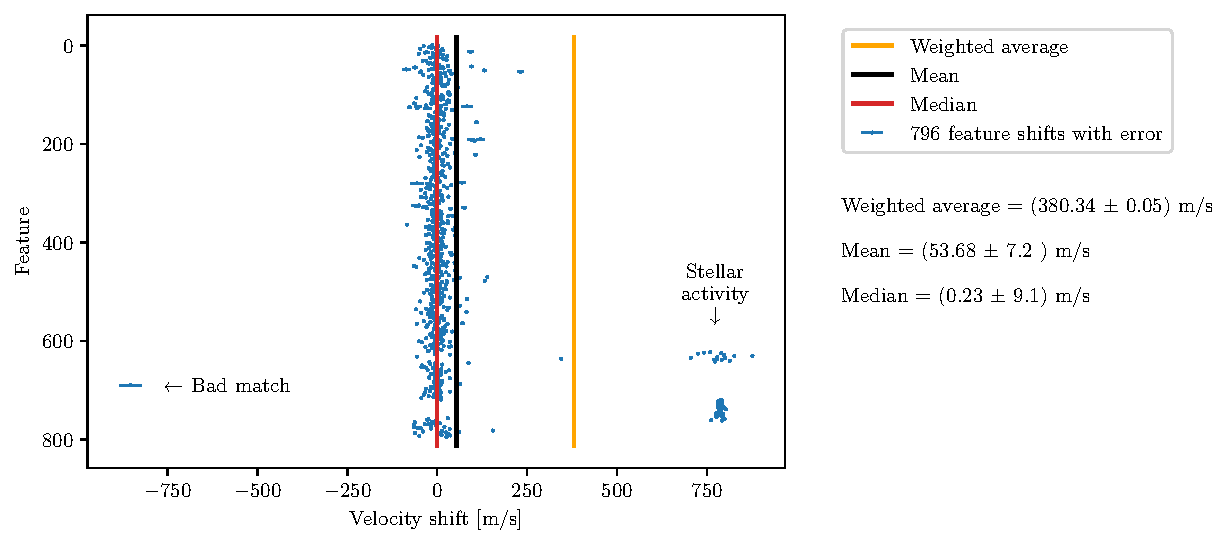
\includegraphics[width=\textwidth]{figures/median-mean-weighted.pdf}
            \caption{Comparison of weighted average, mean and median for computed rv shifts for two observations of HD 34411. The feature on the left side turns out to be a very broad feature, for which the standard data slice is too narrow and therefor yields bad results, (see figure \ref{fig:bad_match_example} in appendix \ref{appendix:RV_extraction}) for details. While the the features on the right side are likely to be caused by some kind of stellar activity.}
        \label{fig:median-mean-weighted-average}
        \end{wide}
    \end{SCfigure}

    The errors however is where my method is falting. Also plotted in figure \ref{fig:median-mean-weighted-average} are the respective errors on the weighted average, the mean and the median. As it is the median that I've decided to work with, it would make sense to use the median error 
    
    $$
        \sigma_{\text{median}} = \frac{\sigma}{\sqrt{N-1}} \times \sqrt{\pi/2}
    $$
    
    for large $N$ where $\sigma$ is the standard deviation,however, it not only comes out very large, but also breaks the propergation of the original errors from the spectrograph, as it essentially is a scaled standard deviation. For the sake of continuing with the analysis I go on with the weighted error, although that in constrast is very small. More on errors in the discussion.
    
    \subsubsection{Extracting relative shifts from over an overconstrained system}
    
    With the devised method we can now compute the relative readial velocity shift between two observations and get out one number with an uncertainty. The next most obvious step would be to compute the shift between observations 1 and 2, 2 and 3, etc. Doing this however leads to correlated results, as the difference between say observation 1 and 10 will depend on all the observations in between, and if there is one bad one, this will affect all the rest. To circumvent this, we can first compute the relative shift between all observations. This will give us an \emph{overconstrained system}, in the sense that there is more information than necessary. All these differences can then be reduced down to a single array, where each shift is relative to all the rest, not only the neighbor. 
    
    Computing the shifts between all observations yields an $N\times N$ upper triangular matrix, where each cell is the shift between observations $i$ and $j$, and thus with a diagonal of zero. I will call this matrix $\Delta V_r^{ij}$, see figure \ref{fig:shift_matrix} for an example.
    
    \begin{SCfigure}[1][!ht]%
        \begin{wide}  
            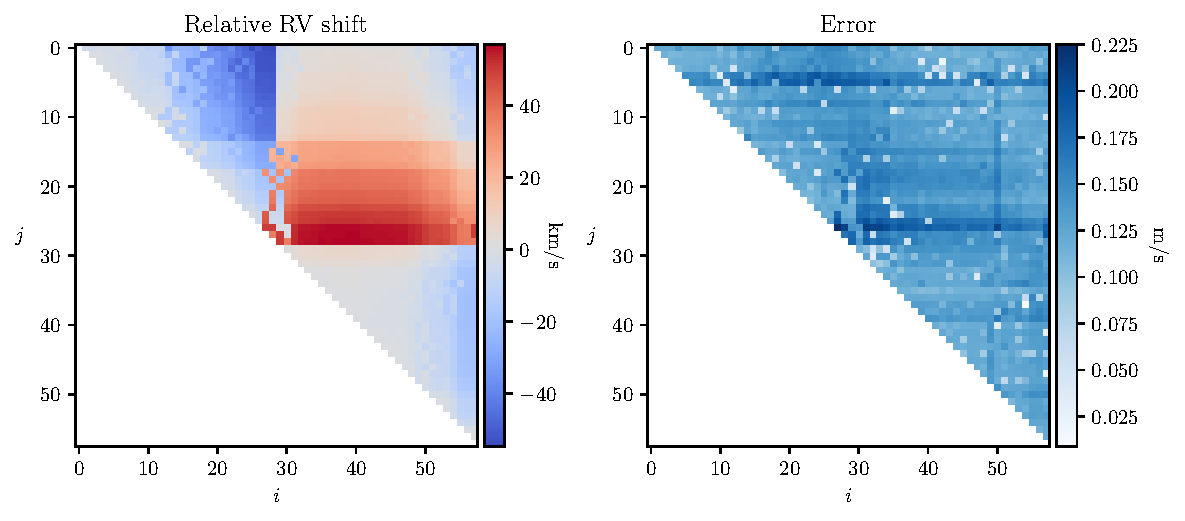
\includegraphics[width=\textwidth]{figures/shfits_matrix_non_bary.pdf}
            \caption{Radial velocity shifts matrix computed for 188 observations for HD34411 using excalibur calibrated but non-barycentric-corrected data (column \texttt{excalibur}). Each cell shows the median radial velocity shift for all features found between observations $i$ and $j$.}
        \label{fig:shift_matrix}
        \end{wide}
    \end{SCfigure}
            
    To reduce the matrix to one array, we can perform another chi2 minimization fit, defined bellow in equation \ref{eq:matrix_reduction_fit}, in which we fit an array of parameters we can call $V_r^i$ of length $N$ (the number of observations), initialized to zero. The chi2 will be at its minimum when it has found an array of velocities $V_r^i$ that best describe all the differences in the matrix $\Delta V_r^{ij}$ and each of the resulting velocities are thus relative not only to its neighbors but to all the other observations as well, thereby avoiding the correlation.
    
    \begin{equation}
        \label{eq:matrix_reduction_fit}
        \chi^{2}=\sum_{i,j = 0}^{N}\left[\frac{ \Delta V_{r}^{ij} - (V_r^i - V_r^j) }{\sigma(\Delta V_{r}^{ij})}\right]^{2} \quad : \quad i < j.
    \end{equation}

    For the sake of illustrating the method, I've analysed non-barycentric-corrected data, that is to say, data in which we should be able to see the movement of the Earth around the center-of-mass of the solar system. That is the data plotted in the matrix in figure \ref{fig:shift_matrix} and the resulting extracted relative radial velocities (the fit parameters $V_r^i$) are plotted in figure \ref{fig:RV_results_non_barycentric} (black), where we see a clear signal of Earth's movement. I've fitted the data with a periodic function and found a  period of $(366.482 \pm 3\mathrm{e}{-6})$ days and an amplitude (the orbital speed of the Earth really) of $(28.132 \pm 9\mathrm{e}{-7})$ km/s. Here there are three things to notice: 1) the errors of the period and amplitude do not cover the discrepancy with the actual values of 365.24 days and 29.78 km/s, 2) the very high chi2 value, and 3) the p-value of zero. These suggest very clearly that my errors are wrong. Nevertheless, the signal is clear and the period and orbital speed found are definitely in the right order of magnitude, from which I confirm that my method in general is working. Comparing with the direct differences between observations 1 and 2, 2 and 3, etc, plotted in blue in figure \ref{fig:RV_results_non_barycentric}, it is also clear that the last step of computing the relative shift between all observatons is vital. 

    \begin{SCfigure}[1][!ht]%
        \begin{wide}  
            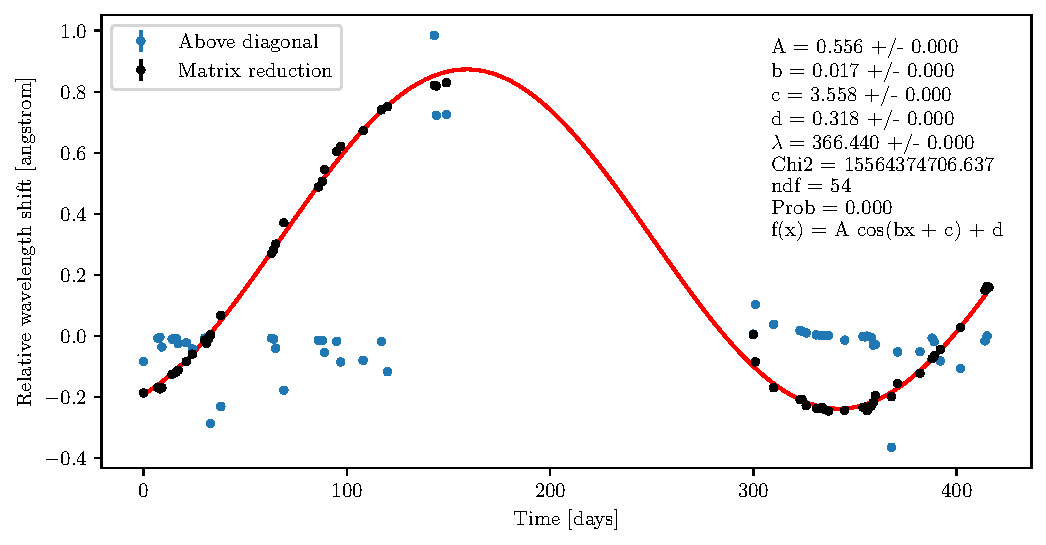
\includegraphics[width=\textwidth]{figures/shift_non_bary_centric.pdf}
            \caption{Final relative radial velocity results for 188 observations of HD 34411 using excalibur calibrated but non-barycentric-corrected data (data column \texttt{excalibur}). Black: values computed through the overconstrained system approach. Blue: above diagonal of $V_r^{ij}$.}
            \label{fig:RV_results_non_barycentric}
        \end{wide}
    \end{SCfigure}

    Although the amount of computations necessary for the described analysis is high, it is possible to execute for 188 observations on a personal computer in about 2 hours. More details are listed in appendix \ref{appendix:run_times}.
    

